%%%%%%%%%%%%%%%%%%%%%%%%%%%%%%%%%%%%%%%%%%%%%%%%%%%%%%%%
%%%%%%%%%%%%%%%%%%%%%%%%%%%%%%%%%%%%%%%%%%%%%%%%%%%%%%%%
\section[Analysis]{Search for a single produced \Tp~decaying into top and Higgs in the full hadronic final state}
\setcounter{tocdepth}{2}

\begin{frame}
\begin{center}
Search for a single produced \Tp~decaying into top and Higgs in the full hadronic final state
\end{center}
\end{frame}


\subsection{Introduction - Analysis Strategy}
\begin{frame}{Introduction - Analysis Strategy}
\vspace{-.2cm}
\begin{columns}

\begin{column}{.50\textwidth}
\begin{block}{}
\begin{itemize}\scriptsize
\item Single produced \Tp~with an associated jet
\item Full hadronic final state: \\ $T'\to t H \to b W^{+} \bar{b} b \to b \bar{b} j j b$
\item Reconstruction of \Tp~mass: $M(5j)$
\item Main challenges:
  \begin{itemize}\scriptsize
  \item Huge backgrounds $\rightarrow$ Mainly QCD and \ttbar
  \item \Tp~reconstruction with high jet multiplicity
  \end{itemize}
\item Fundamental tools for background discrimination:
  \begin{itemize}\scriptsize
  \item B-tagged jets multiplicity
  \item \Tp~reconstruction procedure
  \end{itemize}
\end{itemize}
\end{block}
\end{column}

\begin{column}{.50\textwidth}
\begin{center}
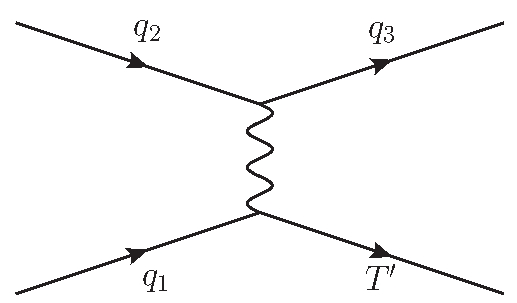
\includegraphics[width=0.9\textwidth]{../figs/Tchannel_T_single.jpg}\\
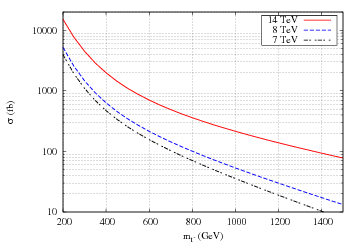
\includegraphics[width=1.0\textwidth]{../figs/pheno_prod_single_tp.png}
\end{center}
\end{column}
\end{columns}

\end{frame}

\begin{frame}{Datasets}
\vspace{-.2cm}

%\begin{table*}[htbH]
\begin{center}
\resizebox{\textwidth}{!}{
\begin{tabular}{|c|c|}
\hline 
Dataset name & Int. Luminosity ($\text{pb}^{-1}$) \\
\hline
/MultiJet/Run2012A-22Jan2013-v1/AOD & 889.4 \\
/MultiJet1Parked/Run2012B-05Nov2012-v2/AOD & 4429.0 \\
/MultiJet1Parked/Run2012C-part1-05Nov2012-v2/AOD & 494.6 \\
/MultiJet1Parked/Run2012C-part2-05Nov2012-v2/AOD & 6654.0 \\
/MultiJet1Parked/Run2012D-part1-10Dec2012-v1/AOD & 5955.1 \\
/MultiJet1Parked/Run2012D-part2-17Jan2013-v1/AOD & 734.0 \\
/MultiJet1Parked/Run2012D-part2-PixelRecover-17Jan2013-v1 & 538.4 \\
\hline
\multicolumn{1}{|r|}{\textit{Total}} & 19694.5 \\
\hline
\end{tabular}
}
%\caption{List of Multijet Primary Dataset used in the analysis and the corresponding integrated luminosity calculated using the golden JSON (Java Script Object Notation) file. The golden JSON file contains the information about the luminosity sections considered as good for all runs. A good luminosity section is defined as a luminosity section where the detector was fully functioning, this is all subsystems were taking data and without problems.  \label{tab:datasets}}
\end{center}
%\end{table*}

%\begin{table*}[htbH]
\begin{center}
\resizebox{\textwidth}{!}{
\begin{tabular}{|c|c|c|}
\hline 
Samples & Cross-Section (pb) & Number of events\\
\hline
QCD\_Pt-120to170\_TuneZ2star\_8TeV\_pythia6 & 16\(\times 10^4\) & 5.9M\\
QCD\_Pt-170to300\_TuneZ2star\_8TeV\_pythia6 & 34\(\times 10^3\) & 5.8M\\
QCD\_Pt-300to470\_TuneZ2star\_8TeV\_pythia6 & 18\(\times 10^2\) & 5.9M\\ 
QCD\_Pt-470to600\_TuneZ2star\_8TeV\_pythia6 & 114 & 3.9M\\
QCD\_Pt-600to800\_TuneZ2star\_8TeV\_pythia6 & 27 & 3.9M\\
QCD\_Pt-800to1000\_TuneZ2star\_8TeV\_pythia6 & 3.5 & 3.9M\\
QCD\_HT-500To1000\_TuneZ2star\_8TeV-madgraph-pythia6 & 84\(\times 10^2\) & 30M\\ 
QCD\_HT-1000ToInf\_TuneZ2star\_8TeV-madgraph-pythia6 & 2\(\times 10^2\) & 14M\\ 
TTJets\_MSDecays\_central\_TuneZ2star\_8TeV-madgraph-tauola & 247.7 [NNLO] & 62M\\
TprimeJetToTH\_\textbf{M-700}\_TuneZ2star\_8TeV-madgraph\_tauola & 143.7 & 99K \\
\hline
\end{tabular}
}
%\caption{List of Monte-Carlo background samples used in the analysis, their corresponding cross-section and their number of events.\label{tab:MCbkg}}
\end{center}
%\end{table*}

\tiny{Signal samples were done with $T'\to tH$ with $H\to\tau^{+}\tau^{-}$ (6\%) and $H\to b\bar{b}$ (94\%). Correction with weight of 0.61 to obtain correct $Br(H\to b\bar{b})=0.57$. }

\end{frame}

\begin{frame}{Event selection}
\vspace{-.2cm}

\begin{columns}

\begin{column}{.55\textwidth}
\begin{block}{Event processing}
\begin{itemize}\scriptsize
  \item Data processed using ``golden'' JSON file: Consider only validated lumi sections
  \item PAT processing
    \begin{itemize}\tiny
    \item Jets reconstructed with PF algorithm and CHS
    \item Jets: \ptg{20} and $|\eta|<5$
    \item At least one good primary vertex: $\text{n.d.o.f.} \ge 4,\; |z|<24 \;\text{cm},\; |\rho|< 2 \;\text{cm}$
    \item Global tag: Calibration and alignment info for data, MC corrected to get close to data conditions
    \end{itemize}
  \item Pile-up corrections: Simulated PU in MC was corrected to observed PU in Data
\end{itemize}
\end{block}
\end{column}

\begin{column}{.45\textwidth}
\vspace{-.9cm}
\begin{figure}[!Hhtbp]
  \begin{center}
    \includegraphics[width=1.0\textwidth]{../figs/Ana/Nvtcs.png}
  \end{center}
\end{figure}
\vspace{-.75cm}
\begin{block}{}
\tiny Number of vertices distribution for data and MC samples. The comparison has been performed after basic selection except number of b-tagged jets (the basic selection is described in the next slides). The gray band correspond to the statistical error of MC samples sum. Normalization of MC samples was done to the 19.7~fb$^{-1}$.
\end{block}
\end{column}

\end{columns}
\end{frame}

\begin{frame}{Basic selection}
\vspace{-.2cm}

\begin{block}{}
  \begin{itemize}\scriptsize
  \item Trigger L1: at least 4 central jets (\etal{3}) with \ptg{32}~or \ptg{36}~or \ptg{40} \\
                    or at least 2 central jets with \ptg{52}~or \ptg{56}~or \ptg{64} \\
                    or events with \HTg{125}~or \HTg{150}~or \HTg{175}
  \item HLT: 6 central jets with a \ptg{20}, 4 with a \ptg{60} and 2 with a \ptg{80}
  \item \textbf{First offline cut}: 2 jets with \ptg{90}, 2 jets with \ptg{70} and 2 jets with \ptg{30}
  \end{itemize}
\end{block}

\begin{columns}
\begin{column}{.50\textwidth}
\vspace{-.2cm}
\begin{block}{}
  \scriptsize \textbf{Second cut}: At least 5 jets with \ptg{30} and \etal{2.5} and at least one additional jet with \ptg{30} and \etal{5} were required
\end{block}

\vspace{-.2cm}
\begin{block}{}
\scriptsize \textbf{Figure}: Distribution of pseudorapidity of the accompanying jet produced with the \Tp. The distribution is taken from the signal MC sample with M=700 \GeVcc~and it is normalized to unity.
\end{block}
\end{column}

\begin{column}{.50\textwidth}
\vspace{-.2cm}
\begin{figure}[!Hhtbp]
  \begin{center}
    \includegraphics[width=1.0\textwidth]{../figs/Ana/SixthJetMCTruth.png}
    %\caption{Distribution of pseudorapidity of the accompanying jet produced with the \Tp. The distribution is taken from the signal MC sample with M=700 \GeVcc~and it is normalized to unity.}
    %\label{fig:SixthJetTp}
  \end{center}
\end{figure}
\end{column}
\end{columns}

\end{frame}

\begin{frame}{}
\vspace{-.2cm}

\begin{columns}
\begin{column}{.50\textwidth}
\begin{block}{}
\scriptsize \textbf{3rd cut}: the leading jet was required to have a \ptg{150}
\end{block}
\vspace{-.2cm}
\begin{block}{}
\scriptsize \textbf{4th cut}: \HTg{550} was required
\end{block}
\vspace{-.2cm}
\begin{block}{}
\scriptsize \textbf{Figure}: Distribution of the $H_{T}$ variable for data and the sum of the MC samples normalized to luminosity. The signal sample (M=700 \GeVcc) is over-imposed on top of the stack of the MC samples. The gray band represents the statistical uncertainties from the sum of the MC background. Reasonable agreement is observed, with the multijet process as the dominant process at this stage. Normalization of samples was done to luminosity.
\end{block}
\end{column}

\begin{column}{.50\textwidth}
\begin{figure}[!Hhtbp]
  \begin{center}
    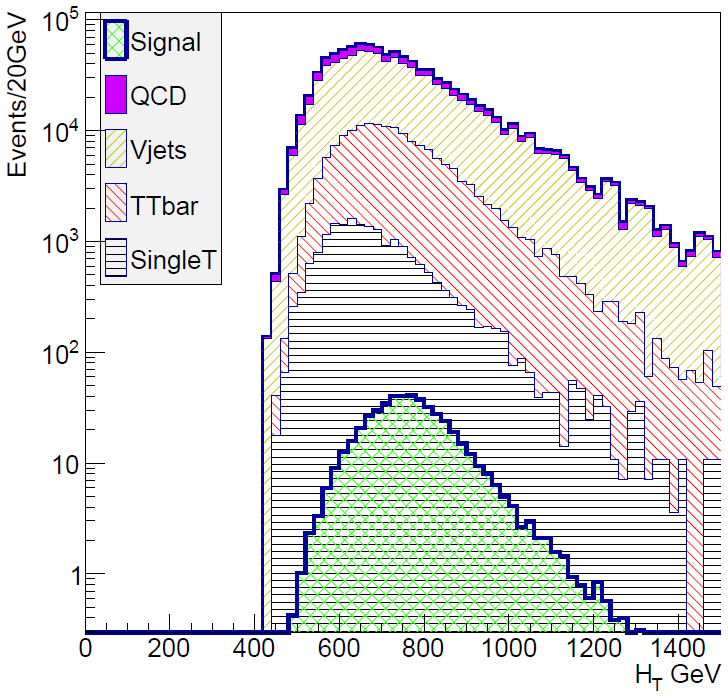
\includegraphics[width=1.0\textwidth]{../figs/Ana/HT.png}
    %\caption{Distribution of the $H_{T}$ variable for data and the sum of the MC samples normalized to luminosity. The signal sample (M=700 \GeVcc) is over-imposed on top of the stack of the MC samples. The gray band represents the statistical uncertainties from the sum of the MC background. Reasonable agreement is observed, with the multijet process as the dominant process at this stage. Normalization of samples was done to luminosity.}
    %\label{fig:HT}
  \end{center}
\end{figure}
\end{column}

\end{columns}
\end{frame}

\begin{frame}{}
\vspace{-.2cm}

\begin{columns}
\begin{column}{.50\textwidth}
\begin{block}{}
\scriptsize \textbf{B-tagging}: CSV (Constrained Secondary Vertex) algorithm $\to$ Multivariate technique that give a discriminator indicating how likely a jet is coming from a b-quark
\textbf{Working points}: Loose, Medium and Tight\\\tiny{CSVL$\to$0.244 \\$\epsilon^{CSVL}_{b}=85$\%, $\epsilon^{CSVL}_{c}=45$\%, $\epsilon^{CSVL}_{l}=10$\% \\CSVM$\to$0.679\\ $\epsilon^{CSVM}_{b}=$70\%, $\epsilon^{CSVM}_{c}=$20\%, $\epsilon^{CSVM}_{l}=$1\% \\CSVT$\to$0.898\\ $\epsilon^{CSVT}_{b}=50$\%, $\epsilon^{CSVT}_{c}=7$\%, $\epsilon^{CSVT}_{l}=0.2$\%}
\end{block}
\vspace{-.2cm}
\begin{block}{}
\scriptsize \textbf{5th cut}: at least 3 CSVM b-tagged jets. Only jets with $|\eta|<=2.4$ considered for b-tagging.
\end{block}
\vspace{-.2cm}
\begin{block}{}
\scriptsize \textbf{Figure}: B-tagged CSVM jet multiplicity for data and MC samples before requiring at least 3 CSVM b-tagged jets. The sum of MC samples is normalized to the integrated luminosity.
\end{block}
\end{column}

\begin{column}{.50\textwidth}
\begin{figure}[!Hhtbp]
  \begin{center}
    \includegraphics[width=1.0\textwidth]{../figs/Ana/NCSVM.png}
    %\caption{B-tagged CSVM jet multiplicity for data and MC samples before requiring at least 3 CSVM b-tagged jets. The sum of MC samples is normalized to the integrated luminosity.}
    %\label{fig:Nb}
  \end{center}
\end{figure}
\end{column}

\end{columns}
\end{frame}



\begin{frame}{Corrections to MC for b-tagging}
\vspace{-.2cm}

\begin{columns}
\begin{column}{.50\textwidth}
\begin{block}{}
\scriptsize Scale factors derived from data/MC comparisons $\to$ $SF^{flavor}_{\eta}(p_{T})$\\
As mean values: $SF^{b\; or\; c}\sim 0.94$ and $SF^{light}\sim 1.06$
\end{block}
\vspace{-.2cm}
\begin{block}{}
\scriptsize In order to apply the SF's a weight per event is calculated\\
$w=\frac{P(\text{DATA})}{P(\text{MC})}$ with \\ \tiny{
$P(\text{MC}) = \prod_{i=\text{tagged}} \varepsilon_i \prod_{j=\text{not tagged}} (1-\varepsilon_j)$\\
$P(\text{DATA}) = \prod_{i=\text{tagged}} \text{SF}_i \varepsilon_i \prod_{j=\text{not tagged}} (1-\text{SF}_j \varepsilon_j)$ \\
}
\end{block}
\vspace{-.2cm}
\begin{block}{}
\tiny B-tagging efficiencies defined as\\
$\varepsilon_f(i,j) = \frac{N_f^\text{b-tagged}(i,j)}{N_f^\text{Total}(i,j)}$ where \\
where $ N_f^\text{Total}(i,j) $ and $ N_f^\text{b-tagged}(i,j) $ are the total number and the number of b-tagged jets, respectively, of flavor $ f $ in the $ (p_\text{T},\eta) $ bin $ (i,j) $ for a given MC sample.
\end{block}
\vspace{-.2cm}
\begin{block}{}
\scriptsize \textbf{Figure}: Distribution of the weights from b-tagging scale factors for all MC samples.
\end{block}
\end{column}

\begin{column}{.50\textwidth}
\begin{figure}[!Hhtbp]
  \begin{center}
    \includegraphics[width=1.0\textwidth]{../figs/Ana/SF_weight.png}
    %\caption{Distribution of the weights from b-tagging scale factors for all MC samples.}
    %\label{fig:SFweight}
  \end{center}
\end{figure}
\end{column}

\end{columns}
\end{frame}

\begin{frame}{\Tp~reconstruction with a $\chi^{2}$ sorting algorithm}
\vspace{-.2cm}
\scriptsize

\begin{itemize}
\item $\chi^{2}$ sorting algorithm used to identify the \Tp~decay products and to reconstruct the Higgs and top candidates
\item $\chi^{2}$ variable defined for each jets combination in an event
\item The combination that minimizes this variable gives the best fit of the objects under reconstruction
\end{itemize}

\begin{equation*}
\chi^{2}=\frac{(M_{H}-M_{bb})^{2}}{\sigma_{H}^{2}}+\frac{(M_{W}-M_{jj})^{2}}{\sigma_{W}^{2}}+\frac{(M_{t}-M_{bjj})^{2}}{\sigma_{t}^{2}}
%\label{eq:chi2def}
\end{equation*}

\begin{itemize}
\item $M_{H}=125$~\GeVcc, $M_{W}=84.06$~\GeVcc, $M_{t}=175.16$~\GeVcc, $\sigma_{H}=12.4$~\GeVcc, and $\sigma_{W}=10.12$~\GeVcc~and $\sigma_{t}=17.35$~\GeVcc. From similar MC studies.
\item For the Higgs reconstruction only CSVM b-tagged jets were considered
\item For the \W~reconstruction all jets with a \ptg{30} were considered
\item For the top reconstruction one b-tagged jet and the pair of jets used for the \W~were utilized
\end{itemize}

\end{frame}

\begin{frame}{}
\vspace{-.2cm}

\begin{columns}
\begin{column}{.50\textwidth}

\begin{figure}[!Hhtbp]
  \begin{center}
    \includegraphics[width=1.0\textwidth]{../figs/Ana/Exclusive_Efficiency_V8.png}
    %\includegraphics[width=0.46\textwidth]{figs/Ana/Inclusive_Efficiency_V8.png}
    %\caption{Reconstruction efficiency by the $\chi^{2}$ algorithm of the Higgs boson, \W~boson, top quark and \Tp, as the ratio of the number of events where the particle was correctly reconstructed to the number of events where jets could be matched to partons [left] and to the total number of events [right]}
    %\label{fig:RecEff}
  \end{center}
\end{figure}

\vspace{-.2cm}
\begin{block}{}
\scriptsize \textbf{Figure}: Reconstruction efficiency by the $\chi^{2}$ algorithm of the Higgs boson, \W~boson, top quark and \Tp, as the ratio of the number of events where the particle was correctly reconstructed to the number of events where jets could be matched to partons.
\end{block}
\end{column}

\begin{column}{.50\textwidth}

\begin{figure}[!Hhtbp]
  \begin{center}
    \includegraphics[width=1.0\textwidth]{../figs/Ana/HundresdsMassChi2Tp.png}
    %\includegraphics[width=0.45\textwidth]{figs/Ana/FiftiesMassChi2Tp.png}
    %\caption{Reconstructed \Tp~mass for all mass points from the $\chi^{2}$ sorting algorithm after basic selection. Each mass point is normalized to luminosity and its corresponding cross section. A gaussian fit of these distributions will be presented afterward in section~\ref{sec:finalsel}, accompanied with a discussion about the resolution on the reconstruction of the \Tp.}
    %\label{fig:RecT}
  \end{center}
\end{figure}

\vspace{-.2cm}
\begin{block}{}
\scriptsize \textbf{Figure}: Reconstructed \Tp~mass for some mass points from the $\chi^{2}$ sorting algorithm after basic selection. Each mass point is normalized to luminosity and its corresponding cross section.
\end{block}
\end{column}

\end{columns}
\end{frame}

\begin{frame}{Selection based on reconstructed objects}
\vspace{-.2cm}
\scriptsize

\begin{columns}
\begin{column}{.50\textwidth}
\vspace{-.2cm}
\begin{block}{}
\tiny
\begin{itemize}
\item Selection optimized via a multidimensional scan of variables 
\item Signal discrimination evaluated by $S/B$, using as signal the $M=700$\GeVcc~mass point, and as background the \ttbar~and QCD\_HT-500To1000
\item Selection has been adjusted to keep at least 10 signal events, for the 700~\GeVcc~mass point, after the full selection
\item \textbf{Data/MC plots are shown for illustration, but final background estimation is derived from data}
\end{itemize}
\end{block}
\vspace{-.2cm}
\begin{block}{}
\scriptsize \textbf{1st criterion}: $\chi^{2}<8$
\end{block}
\vspace{-.2cm}
\begin{block}{}
\scriptsize \textbf{Figure}: Distribution of the $\chi^{2}$ variable for data and MC samples. The signal sample used has a \Tp~mass of 700 \GeVcc. Backgrounds present higher values than the signal. The sum of MC is normalized to the integrated luminosity.
\end{block}
\end{column}

\begin{column}{.50\textwidth}
\begin{figure}[!Hhtbp]
  \begin{center}
    \includegraphics[width=1.0\textwidth]{../figs/Ana/chi2Nm1.png}
    %\caption{Distribution of the $\chi^{2}$ variable for data and MC samples. The signal sample used has a \Tp~mass of 700 \GeVcc. Backgrounds present higher values than the signal. The sum of MC is normalized to the integrated luminosity. }
    %\label{fig:chi2}
  \end{center}
\end{figure}
\end{column}

\end{columns}

\end{frame}

\begin{frame}{}
\vspace{-.2cm}
    \begin{block}{}\scriptsize
      \textbf{2nd criterion}: $\Delta R(bb)<1.2$\\
      \textbf{3rd criterion}: Higgs candidate mass between 105 and 145 \GeVcc
    \end{block}

\vspace{-.5cm}
\begin{columns}
\begin{column}{.50\textwidth}
\begin{figure}[!Hhtbp]
  \begin{center}
    \includegraphics[width=0.9\textwidth]{../figs/Ana/DRbbNm1.png}
  \end{center}
\end{figure}

\vspace{-.7cm}
    \begin{block}{}\tiny
      $\Delta R$ of the 2 b-tagged jets used to reconstruct the Higgs candidate after $\chi^{2}$ cut.
    \end{block}
\end{column}

\begin{column}{.50\textwidth}
\begin{figure}[!Hhtbp]
  \begin{center}
    \includegraphics[width=0.9\textwidth]{../figs/Ana/HMNm1.png}
  \end{center}
\end{figure}

\vspace{-.7cm}
    \begin{block}{}\tiny
      Distribution for $M(H_{cand})$ for data and the sum of Monte Carlo samples. All others selection criteria are applied up to this one.
    \end{block}
\end{column}

\end{columns}

\end{frame}


\begin{frame}{}
\vspace{-.2cm}
    \begin{block}{}\scriptsize
      \textbf{4th criterion}: $(M(top^{2nd})+M(W^{2nd}))/M(H)>6.8$\\
      \textbf{5th criterion}: $\Delta R (T' j^{6})>4.8$\\
      \textbf{6th criterion}: $H_{T}>0.67$
    \end{block}

\vspace{-.5cm}
\begin{columns}
\begin{column}{.50\textwidth}
\begin{figure}[!Hhtbp]
  \begin{center}
    \includegraphics[width=0.8\textwidth]{../figs/Ana/M2HPNm1.png}
  \end{center}
\end{figure}

\vspace{-.7cm}
    \begin{block}{}\tiny
      Distribution of $(M(top^{2nd})+M(W^{2nd}))/M(H)$ for data and the sum of the Monte Carlo samples. Selection criteria are applied up to Higgs mass cut. The low statistics in the multijet (QCD) MC sample is visible at this stage.
    \end{block}
\end{column}

\begin{column}{.50\textwidth}
\begin{figure}[!Hhtbp]
  \begin{center}
    \includegraphics[width=0.8\textwidth]{../figs/Ana/DRTp6JNm1.png}
  \end{center}
\end{figure}

\vspace{-.7cm}
    \begin{block}{}\tiny
      Distributions for $\Delta R (T' j^{6})$  for data and the sum of Monte Carlo samples. All others criteria are applied up to this one. The low statistics in the multijet (QCD) MC sample is visible at this stage.
    \end{block}
\end{column}

\end{columns}

\end{frame}

\begin{frame}{Selection optimization}
\vspace{-.2cm}

\begin{table}[htbH]
\begin{center}
\resizebox{\textwidth}{!}{
\begin{tabular}{|c|c|c|}
\hline 
Cut & $S/B$ & $S/\sqrt{S+B}$ \\
\hline
$\chi^{2}<8$ & $3.4\ex{-2} \pm 2.85\ex{-3}$  & $ 0.96 \pm 0.05$  \\
$\Delta R(bb)<1.2$ & $4.76\ex{-2} \pm 4.52\ex{-3}$ & $1.10 \pm 0.07$  \\
%$1.6<\Delta R (W_{cand} H_{cand})<4.0$ & $4.82\ex{-2} \pm 4.59\ex{-3}$  & $1.10 \pm 0.07$  \\
$105$ \GeVcc~$< M(H_{cand}) < 145$ \GeVcc~& $6.37\ex{-2} \pm 6.74\ex{-3}$  & $1.22 \pm 0.08$  \\
$(M(top^{2nd})+M(W^{2nd}))/M(H_{cand})>6.8$ & $0.15 \pm 0.03$  & $1.45 \pm 0.16$  \\
$\Delta R (T j^{6})>4.8$ & $0.42 \pm 0.19$  & $1.67 \pm 0.32$  \\
Relative $H_{T}>0.67$ & $1.16 \pm 0.17$  & $2.13 \pm 0.17$  \\
\hline
\end{tabular}
%\caption{$S/B$ and $S/\sqrt{S+B}$ from MC samples for each step of the selection after reconstruction of resonances with the $\chi^{2}$ sorting algorithm. Only $M=700$ \GeVcc~signal, \ttbar~and QCD\_HT-500To1000 MC samples were used. \label{tab:Estimators}}
}
\end{center}
\end{table}

\vspace{-.2cm}
    \begin{block}{}\scriptsize
      $S/B$ and $S/\sqrt{S+B}$ from MC samples for each step of the selection after reconstruction of resonances with the $\chi^{2}$ sorting algorithm. Only $M=700$ \GeVcc~signal, \ttbar~and QCD\_HT-500To1000 MC samples were used.
    \end{block}

\end{frame}

\begin{frame}{Trigger efficiency}
\vspace{-.2cm}

\begin{columns}
\begin{column}{.50\textwidth}
   \begin{block}{}\scriptsize
     \begin{itemize}
     \item Prescaled trigger requiring \HTg{400} as reference.
     \item The \pt~of the 6th leading jet has been used to parametrize the trigger efficiency.
     \item Efficiency = number of events passing analysis and reference triggers / number of events passing only HLT\_HT400
     \end{itemize}
    \end{block}

\vspace{-.2cm}
    \begin{block}{}\tiny
      \textbf{Figure}: Efficiency in data and the MC signal samples for events passing trigger bit HLT\_Dijet80\_Dijet60\_Dijet20 with respect to trigger bit HLT\_HT400 after full selection. This efficiency is parametrized as function of the 6$^{th}$ jet $p_{T}$. The dispersion observed is about 10\% between data and signal MC samples, while only about 4\%  for \ttbar. Efficiencies for signal MC samples with \Tp~masses equal to 600, 700, 800, 900 and 1000~\GeVcc~are shown with \ttbar~and data.
    \end{block}
\end{column}

\begin{column}{.50\textwidth}
\begin{figure}[!Hhtbp]
  \begin{center}
    \includegraphics[width=1.0\textwidth]{../figs/Ana/Trigger_Eff_hundreds_FullSel.png}
    %\includegraphics[width=0.45\textwidth]{../figs/Ana/Trigger_Eff_fifties_FullSel.png}
    %\caption{Efficiency in data and the MC signal samples for events passing trigger bit HLT\_Dijet80\_Dijet60\_Dijet20 with respect to trigger bit HLT\_HT400 after full selection. This efficiency is parametrized as function of the 6$^{th}$ jet $p_{T}$. The dispersion observed is about 10\% between data and signal MC samples, while only about 4\%  for \ttbar. This efficiency is parametrized as function of the 6$^{th}$ jet $p_{T}$. Efficiencies for signal MC samples with \Tp~masses equal to 600, 700, 800, 900 and 1000~\GeVcc~are shown with \ttbar~and data [left]. Efficiencies for signal MC samples with \Tp~masses equal to 650, 750, 850 and 950~\GeVcc~are shown with \ttbar~and data [right].}
    \label{fig:TrigEffPostMH}
  \end{center}
\end{figure}
\end{column}

\end{columns}


\end{frame}